
\documentclass{include/thesisclass3}

\SelectLanguage{ngerman}
\usepackage{float}


% Titlepage settings
\newcommand{\praktikum}{Praktikum moderne Physik}
\newcommand{\autora}{Jens Schäfer}
\newcommand{\autorb}{Jan van der Linden}
\newcommand{\maila}{schaferjens92@gmail.com}
\newcommand{\mailb}{jan.vdlinden95@gmail.com}
\newcommand{\topic}{Versuch}
\newcommand{\ptime}{Datum}


% Shortcuts
\newcommand{\cc}{\cdot}
\newcommand{\rk}{\rangle}
\newcommand{\lk}{\langle}
\newcommand{\df}{\rightarrow}
\newcommand{\la}{\lambda}
\newcommand{\dd}{{\rm d}}
\newcommand{\ehm}{\mathbbm{1}}
\newcommand{\p}{\partial}
\newcommand{\soll}{\overset{!}{=}}
\newcommand{\D}{\Delta}
\newcommand{\eps}{\epsilon}
\newcommand{\vektor}[3]{\begin{pmatrix} #1 \\ #2 \\ #3 \end{pmatrix}}
\newcommand{\vektorz}[2]{\begin{pmatrix} #1 \\ #2 \end{pmatrix}}
\newcommand{\Mat}[9]{\begin{pmatrix}#1&#2&#3\\#4&#5&#6\\#7&#8&#9\end{pmatrix}}
\newcommand{\Matz}[4]{\begin{pmatrix}#1&#2\\#3&#4\end{pmatrix}}



\begin{document}

	\FrontMatter
	% coordinates for background border
\newcommand{\diameter}{20}
\newcommand{\xone}{-15}
\newcommand{\xtwo}{160}
\newcommand{\yone}{15}
\newcommand{\ytwo}{-253}




\begin{titlepage}
    % background border
    \begin{tikzpicture}[overlay]
    \draw[color=gray]
            (\xone mm, \yone mm)
      -- (\xtwo mm, \yone mm)
    arc (90:0:\diameter pt)
      -- (\xtwo mm + \diameter pt , \ytwo mm)
        -- (\xone mm + \diameter pt , \ytwo mm)
    arc (270:180:\diameter pt)
        -- (\xone mm, \yone mm);
    \end{tikzpicture}



    % KIT image and sign for faculty of physics
    \begin{textblock}{10}[0,0](4.5,2.5)
        \includegraphics[width=.25\textwidth]{include/kitlogo.pdf}
    \end{textblock}
    

    % horizontal line
    \begin{textblock}{10}[0,0](4.2,3.1)
        \begin{tikzpicture}[overlay]
        \draw[color=gray]
                (\xone mm + 5 mm, -12 mm)
          -- (\xtwo mm + \diameter pt - 5 mm, -12 mm);
        \end{tikzpicture}
    \end{textblock}



    % begin of text part
    \changefont{phv}{m}{n}    % helvetica
    \centering



    % thesis topic (en and ge)
    \vspace*{3cm}
    \Huge\praktikum\\



    % author name and institute
    \vspace*{5cm}
    
    \huge\topic\\






    % examiners (Referenten)
    \vspace*{3cm}
    \Large
    \begin{center}
        \begin{tabular}[ht]{l c l } 
  \autora & \hfill & \textit{\maila} \\
\autorb & \hfill & \textit{\mailb} \\
        
        \end{tabular}
    \end{center}



    % working time
    \vspace{2cm}
    \begin{center}
        \large{Durchgeführt am}: \ptime
    \end{center}



    % lowest text blocks concerning the KIT
    \begin{textblock}{10}[0,0](4,16.8)
        \tiny{KIT -- Universität des Landes Baden-Württemberg und nationales %
              Forschungszentrum in der Helmholtz-Gemeinschaft}
    \end{textblock}
    \begin{textblock}{10}[0,0](14,16.75)
        \large{\textbf{www.kit.edu}}
    \end{textblock}
\end{titlepage}

	\tableofcontents                  
	\newpage
	\MainMatter

%Protokollstart

\chapter{Theoretische Grundlagen}
\section{Ziel des Experiments}
In diesem Experiment soll anhand eines Modells untersucht werden, wie ein Antibiotikum auf eine Zellmembran wirkt. Dazu wird ein Präparat einer Lipid Doppelmembran angefertigt und einem Antibiotikum (Gramicidin A) ausgesetzt. Durch das Antibiotikum werden Ionenkanäle in der Membran gebildet und somit Kationenfluss ermöglicht. Für eine Zelle bedeutet dies, dass ihr Potential zusammenbricht und sie stirbt.\\
\\
Hier soll die Generierung einer solchen Membran beobachtet werden und das Entstehen sowie die Beschaffenheiten der Ionenkanäle näher untersucht werden.


\section{Black Lipid Membran Methode}

Bei der Black Lipid Membran Methode ist eine speziell geformte Küvette aus PTFE Herzstück des Aufbaus. Zwei Tanks werden durch eine Trennwand abgeschirmt die eine kleine, kreisrunde Öffnung mit abgerundeten, weichen Kanten beinhaltet. Eine Wand der Küvette beinhaltet ein Fenster wodurch die Öffnung beobachtet werden kann. In dieser Öffnung werden die Peptide aufgetragen. Sie bilden einen geschlossenen, zunächst undurchdringlichen Film. Die beiden Tanks werden mit Elektrolüten gefüllt und Ag/AgCl-Elektroden ausgestattet. Durch die Zerstörung der Lipidschicht kann nun ein elektrischer Strom die Barriere überwinden und gemessen werden \ref{aufbau}.\\
\begin{figure}[ht]
	\begin{center}
		\includegraphics{images/experiment.png}
		\caption{Experimenteller Aufbau}
		\label{aufbau}
	\end{center}
\end{figure}
Die Natur der Lipide gibt vor, dass sie sich innerhalb einer Grenzschicht parallel anordnen. Dabei zeigen in wässriger Lösung die hydrophilen Köpfe nach außen, nach innen gerichtet sind die hydrophoben Fettsäureketten, die sich mit den Fettsäuren der gegenüberliegenden Grenzschicht anziehen. So bauen die Lipide eine Kette mit einer gewissen Oberflächenspannung auf und trennen die Tanks dicht ab \ref{double}. Die Dicke wird somit ziemlich gut konstant gehalten und die Doppelschicht besitzt isolierende Eigenschaften. Daher kann man die Trennlinie in guter Näherung als Plattenkondensator ansehen.\\
\begin{figure}[ht]
	\begin{center}
		\includegraphics{images/lipid-doublelayer.png}
		\caption{Lipid-Doppelschicht}
	\label{double}
	\end{center}
\end{figure}
Die Dicke der Leptidschicht kann anhand ihrer optischen Eigenschaften eingeordnet werden. Eine weiße Schicht hat eine Dicke d gegenüber der Wellenlänge $\lambda \ll d$, bei $\lambda \approx d$ zeichnen sich newtonsche Ringe ab und für $\lambda \gg d$ erscheint die Oberfläche schwarz. Die Membran wird bei sehr geringer Dicke bevorzugt untersucht um die Kondensatornäherung bestmöglich zu erfüllen, daher der auch die Namensgebung.

\section{Gramicidin A}
Gramicidin A ist ein Peptid-Antibiotikum. Diese bestehen in der Regel aus 10 bis 50 Aminosäuren und können mit Zellmembranen interagieren.\\
Im Körper werden Peptid-Antibiotika selbst generiert und werden benutzt, um infizierte Zellen zu zerstören.  Um dies zu bewerkstelligen integrieren sie sich in die Zellmembran und ermöglichen es somit auf verschiedenen Wegen, Ionen in die Zelle einzudringen. Bei Gramicidin A geschieht dies durch die Bildung von  Kanälen in der Membran Diese haben Durchmesser von etwa $3 - 4~\si{\AA}$. Durch den Fluss von Kationen in die Zelle wird damit ihr elektrochemisches Gleichgewicht gestört und sie stirbt ab.\\
In diesem Experiment wird die Penetration der Zelle durch die Lipid Doppelmembran simuliert; nachdem sich die Membran gebildet hat, ist kein Stromfluss mehr durch die Elektroden möglich. Nach Zugabe von Gramicidin A können in der Membran Kanäle gebildet werden, welche Stromfluss ermöglichen. Dies ist gleichbedeutend mit einer erfolgreichen Bekämpfung und Zerstörung einer infizierten Zelle im Körper mittels eines Peptid-Antibiotikums.


%hab keine lust die verschiedenen penetrationsmethoden zu beschreiben, juckt ja auch keinen.


\section{Generierung der Membran}
Als erster Versuchsschritt soll eine Membran generiert werden. Dazu wird eine geringe Menge an Glycerol Monooleat in Tetradecan auf die Öffnung gebracht. Dadurch wird eine Lipide Doppelmembran generiert. Dies soll optisch beobachtet werden; die Farbe der Membran verändert sich, je nach Dicke bis sie komplett schwarz wird.\\
Für die fertige Membran kann die Leitfähigkeit sowie die Kapazität und die Dicke bestimmt werden. \\Die Leitfähigkeit $G$ kann über den gemessenen Strom durch die Membran und die angelegte Spannung bestimmt werden über $G = \frac{I}{U}$. \\Um die Kapazität zu bestimmen kann angenommen werden, dass die Doppelmembran  sich im Stromkreislauf wie ein Plattenkondenstator verhält. Daher ist der übliche Zusammenhang für einen Plattenkondensator gültig:
\begin{equation}
C = e_0e_m \frac{A}{d}
\end{equation}

% Dicke, spez. Membrankapazität, Membranwiderstand, Durchbruchspannung, max. E-Feld


\section{Einzelkanal Messungen}
Gibt man nur sehr geringe Mengen Gramicidin A in die Lösung so bilden sich auch nur sehr wenige Kanäle in der Membran. Dies wird durch einen quantisierten Stromverlauf sichtbar womit die Anzahl der aktiven Kanäle und auch der Stromfluss pro Kanal bestimmbar sind.\\
Ebenso kann durch die Aufnahme eines Stromhistogramms die Lebensdauer eines Kanals bestimmt werden.\\
Desweitern gilt zu überprüfen, ob das Ohmsche Gesetz hier erfüllt ist:
\[ I_M = \lambda_M \cc V_M\]
mit $I_M$ dem Strom und $\lambda_M$ der Leitfähigkeit durch die Membran, sowie $V_M$ die Potentialdifferenz der beiden Elektrolyte auf beiden Seiten der Membran.

%Ohms Gesetz

\section{Multikanal Messungen}
Erhöht man die Konzentration des Gramicidin A so öffnen und schließen sich viel mehr Kanäle und eine Vermessung der einzelnen Kanäle ist nicht mehr möglich. Jedoch besteht die Möglichkeit Aussagen über das Öffnen und Schließen der Kanäle, also die Lebenszeit durch eine Autokorrelationsfunktion zu treffen.\\
Dazu soll ein Stromhistogramm aufgenommen werden und über Autokorrelation verglichen werden. Dazu verschiebt man den Verlauf des Histogramms in der Zeit und berechnet die Korrelation des verschobenen Verlaufs mit dem ursprünglichen Verlauf. Ein hoher Korrelationswert deutet auf eine, sich wiederholende Struktur hin, woraus die Halbwertszeit bestimmt werden kann.

\section{Weitere Analysen}

% Bestimmung des Dissoziation der Ratenkoeffizienten des Antibiotikum (?????)
% Kanalleitfähigkeit
% Teilchenfluss






\chapter{Versuchsablauf}
Der Versuchsablauf orientiert sich an der Lösung der im BLM-Dokument unter \grqq 2. Questions and to dos\grqq  ~aufgelisteten Fragestellungen
\section{Lipid membrane preparation}

Preparation einer Lipid-Doppelschicht mit Glycerol-monooleate in Tetradecanelektrische und optische darstellung der Lipid-Doppelschicht\\

Bestimmen der Membrankapazität, der spezifischen Membrankapazität und der Membrandicke\\ 

Bestimmen des Membranwiderstandes\\ 

Bestimmen der Schwellspannung und des maximalen E-Feldes

\section{Measurement of single channels}
Ändern der Leitfähigkeit für Gleichstrom mittels kleiner Gramicidin A-konzentrationen\\

Bestimmen des Stromes und der mittleren Lebensdauer eines Channels mittels des Stromhistogrammes\\

Überprüfen des ohmschen Gesetzes mit einem einzelnen Channel\\

\section{Measurement of multiple channels}

Darstellen der Channelformierung mit einer hohen Gramicidin A-konzentration\\

Bestimmen des Stromes eines einzelnen Channels mittels des Stromhistogrammes\\

Bestimmen des Stromes eines einzelnen Channels und der mittleren Öffnungsdauer eines Channels mittels der analyse der autokorrelationsfunktion des Stromrauschens

\section{Further questions}

Gegenüberstellen der verschiedenen methoden und der Resultate\\

den check ich nich\\

Darstellen der Leitfähigkeit einzelner Channels von Gramicidin A kanälen\\

Berechnung des Partikelflusses (=Ionen/Sekunde) durch einen Gramicidin A-kanal



\chapter{Versuchsauswertung Teil 1}
\section{Membran auftragen}
Um die BLM zu Präparieren wurde mit einem Teflonstab ein dünner Film der Peptidschicht auf die Kapilare aufgetragen. Die anfangs dicke Schicht wird durch sanftes abstreifen, klopfen oder rühren verjüngt. Durch die Kamera kann man dabei die Ausprägung der newtonschen Ringe beobachten. In Abbildung \ref{Reihe} ist Kapilare mit unterschiedlich dicken Lipidmembranen zu sehen. Links ist die Membran dick genug, um Licht hindurch zu lassen, sie erscheint durchsichtig. Die mittlere ist im Bereich der Wellenlängen von sichtbarem Licht und bildet damit newtonsche Ringe aus. Bei der dritten Aufnahme ist die Membran im Begriff sich auszudünnen, man erkennt die Lichtunterdrückung rechtsseitig und damit die Schwarzfärbung.
\begin{figure}[ht]
	\begin{center}
		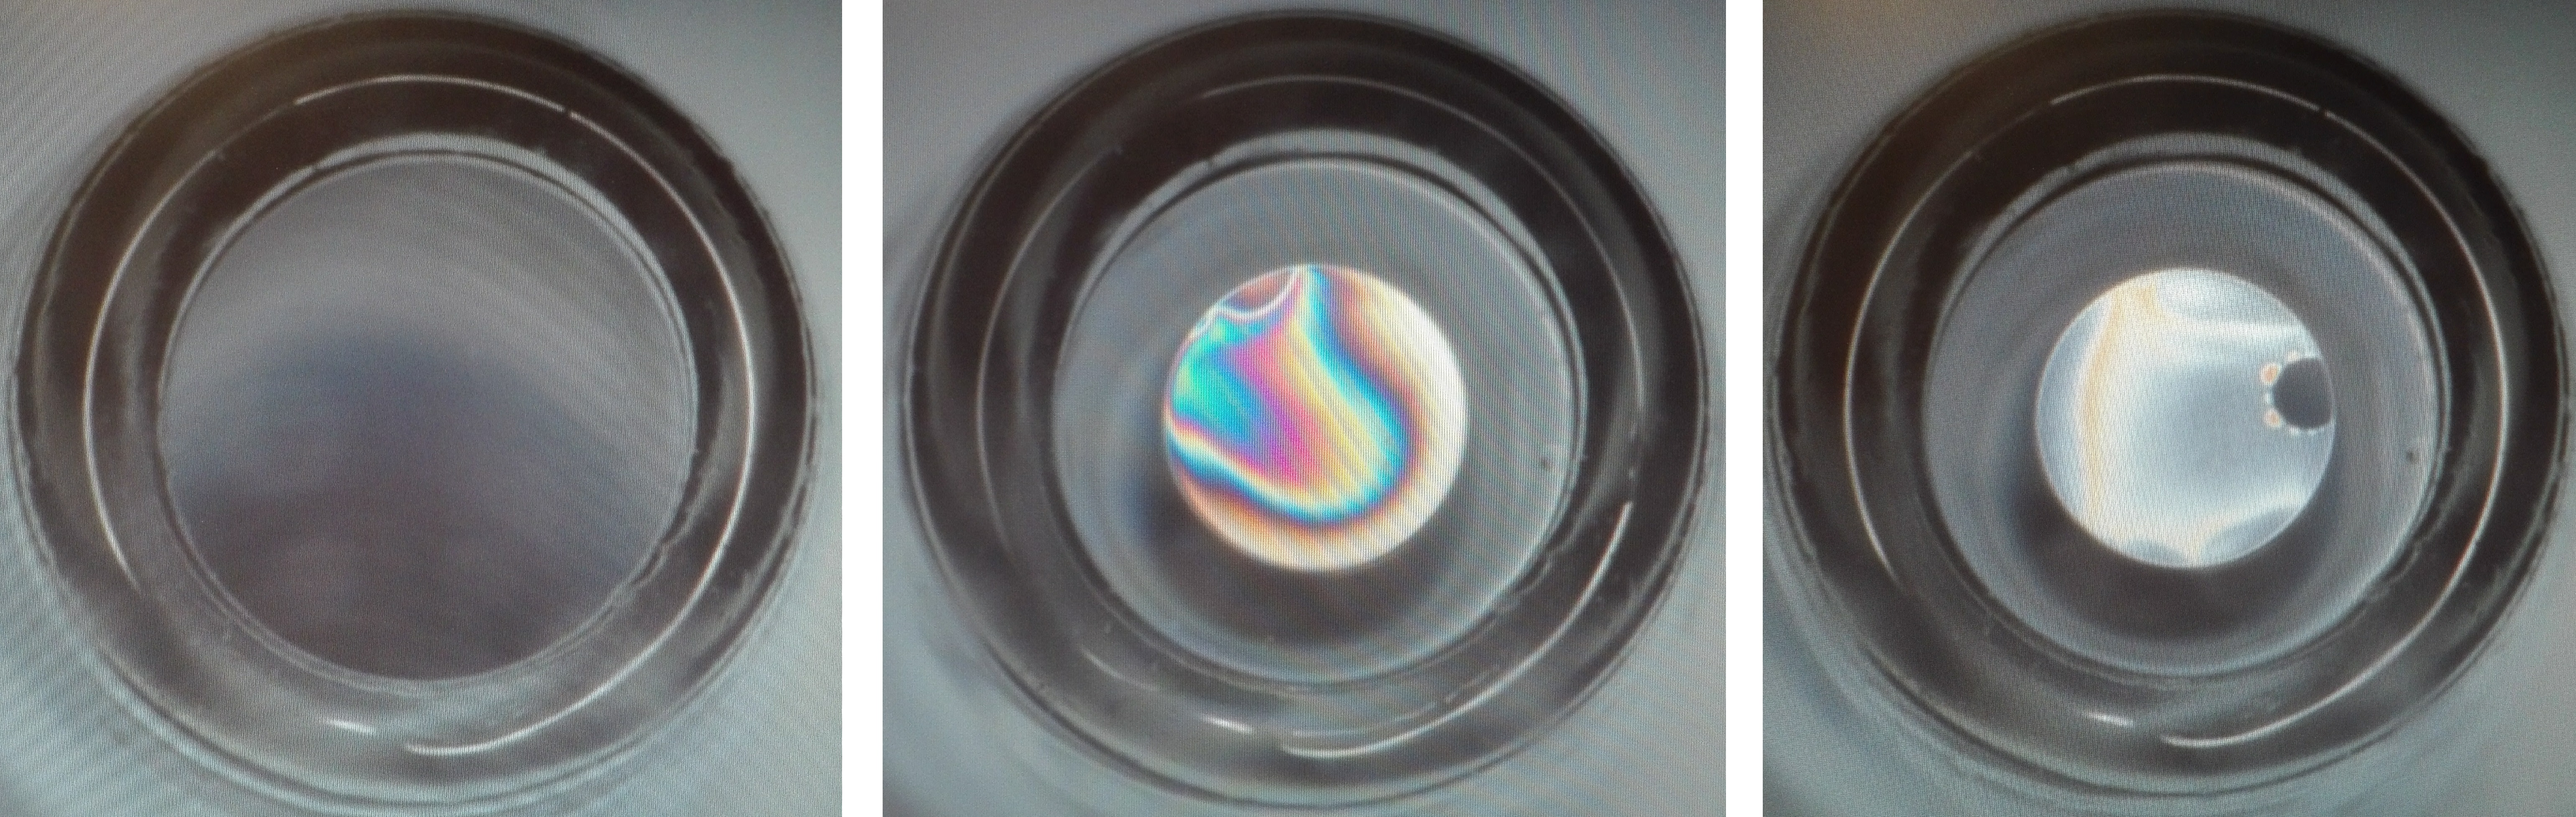
\includegraphics[width=1\textwidth]{images/Reihe.png}
		\caption{Lichtdurchlässige Membran (l), Newtonsche Ringe (m), BLM (r)}
		\label{Reihe}
	\end{center}
\end{figure}
\section{Membranfläche}
Um die Fläche der Membran zu bestimmen untersuchen die Kameraaufnahmen. Relevant für die untersuchten Prozesse ist nur jener dünne und schwarze Anteil der Membran. Hierzu dient die Aufnahme \ref{Perle}. Bei der Untersuchung der Verhältnisse aus Pixel/Milimeter für den Kapilaraußen/ und -innendurchmesser fällt auf, dass das Verhältniss mit zunehmendem Abstand von der optischen Achse zunimmt. Dieser Effekt ist der Krümmung der Linse verschuldet und wird in der Optik als kissenförmige Verzeichnung bezeichnet \ref{Verzeichung}.
\begin{figure}[ht]
	\begin{center}
		\includegraphics[width=0.4\textwidth]{images/Verzeichnung.png}
		\caption{https://upload.wikimedia.org/wikipedia/commons/0/0a/Verzeichnung3.png}
		\label{Verzeichnung}
	\end{center}
\end{figure}
Da die Verzeichnung allerdings exponentiel mit dem Abstand zur Bildmitte zunimmt und die Verhältnisse zwischen Außen- und Innenwand nur 5,6\% (\ref{tab-ratio}) betragen, können wir im inneren der Kapilare lineare Verhältnise voraussetzen, insbesondere da die BLM recht zentriert in der Kapilare auftreten.
Um den Fehler minimal zu halten, rechnet man mit dem Verhältnis des Innendurchmessers um den BLM-Durchmesser zu bestimmen. Die Zahlen sind in Tabelle \ref{tab-ratio} eingetragen.
\begin{align*}
	\text{Verhältniss Au\ss en:\qquad} &1345,16\\
	\text{Verhältniss Innen:\qquad} &1273,91\\
	\text{Differenz:\qquad} & 71,3 \qquad= \quad 5,59\%
\end{align*}
\begin{table}[]
	\centering
	\caption{Vermessung von Kapilare und BLM}
	\label{tab-ratio}
	\begin{tabular}{llll}
		& Au\ss en   & Innen     & BLM     \\
		\O  (Pixel) & 2085    & 1465    & 441     \\
		\O  (Milimeter)       & 1,55    & 1,15    & $\approx$ 0,346   \\
		p/mm            & 1345,16 & 1273,91 & $\approx$ 1273,91
	\end{tabular}
\end{table}
\begin{figure}[ht]
	\begin{center}
		\includegraphics[width=0.4\textwidth]{images/Perle2.png}
		\caption{Vermessung von Kapilare und BLM}
		\label{Perle}
	\end{center}
\end{figure}

\section{Kapazität}
Bei der Messung der Kapazität wird eine Wechselspannung von $U_{C0}=5mV$ mit $F=50Hz$ an die Elektroden angelegt. Dabei wird die Spannung über der Membran aufgezeichnet und ein Widerstand $R_1=100k\Omega$ in Reihe geschalten. Abbildung \ref{oszi} zeigt die zugehörige Oszilloskopaufnahme, man erkennt darauf, dass die Analogie zum Kondensator sehr gut erfüllt ist. Eingezeichnet wurde die Peakspannung von $U_0 = 7,5$V und die geometrisch konstruierte Strecke von 53 Pixel, die der charakteristischen Zeit $\tau$ entspricht, während der die Spannung auf $U_0/\textit{e}\approx 2,8V$ abfällt.
\begin{align*}
\tau = \frac{53}{1250} \cdot 1/50 Hz= 0,84 ms\\
C=\tau / R_1 = 0,84ms \cdot 100k\Omega = 8,4 nF
\end{align*}
\begin{figure}[ht]
	\begin{center}
		\includegraphics[width=1\textwidth]{images/measure.png}
		\caption{Vermessung von Kapilare und BLM}
		\label{oszi}
	\end{center}
\end{figure}




\begin{itemize}
\end{itemize}





\end{document}
